\documentclass[1p]{elsarticle_modified}
%\bibliographystyle{elsarticle-num}

%\usepackage[colorlinks]{hyperref}
%\usepackage{abbrmath_seonhwa} %\Abb, \Ascr, \Acal ,\Abf, \Afrak
\usepackage{amsfonts}
\usepackage{amssymb}
\usepackage{amsmath}
\usepackage{amsthm}
\usepackage{scalefnt}
\usepackage{amsbsy}
\usepackage{kotex}
\usepackage{caption}
\usepackage{subfig}
\usepackage{color}
\usepackage{graphicx}
\usepackage{xcolor} %% white, black, red, green, blue, cyan, magenta, yellow
\usepackage{float}
\usepackage{setspace}
\usepackage{hyperref}

\usepackage{tikz}
\usetikzlibrary{arrows}

\usepackage{multirow}
\usepackage{array} % fixed length table
\usepackage{hhline}

%%%%%%%%%%%%%%%%%%%%%
\makeatletter
\renewcommand*\env@matrix[1][\arraystretch]{%
	\edef\arraystretch{#1}%
	\hskip -\arraycolsep
	\let\@ifnextchar\new@ifnextchar
	\array{*\c@MaxMatrixCols c}}
\makeatother %https://tex.stackexchange.com/questions/14071/how-can-i-increase-the-line-spacing-in-a-matrix
%%%%%%%%%%%%%%%

\usepackage[normalem]{ulem}

\newcommand{\msout}[1]{\ifmmode\text{\sout{\ensuremath{#1}}}\else\sout{#1}\fi}
%SOURCE: \msout is \stkout macro in https://tex.stackexchange.com/questions/20609/strikeout-in-math-mode

\newcommand{\cancel}[1]{
	\ifmmode
	{\color{red}\msout{#1}}
	\else
	{\color{red}\sout{#1}}
	\fi
}

\newcommand{\add}[1]{
	{\color{blue}\uwave{#1}}
}

\newcommand{\replace}[2]{
	\ifmmode
	{\color{red}\msout{#1}}{\color{blue}\uwave{#2}}
	\else
	{\color{red}\sout{#1}}{\color{blue}\uwave{#2}}
	\fi
}

\newcommand{\Sol}{\mathcal{S}} %segment
\newcommand{\D}{D} %diagram
\newcommand{\A}{\mathcal{A}} %arc


%%%%%%%%%%%%%%%%%%%%%%%%%%%%%5 test

\def\sl{\operatorname{\textup{SL}}(2,\Cbb)}
\def\psl{\operatorname{\textup{PSL}}(2,\Cbb)}
\def\quan{\mkern 1mu \triangleright \mkern 1mu}

\theoremstyle{definition}
\newtheorem{thm}{Theorem}[section]
\newtheorem{prop}[thm]{Proposition}
\newtheorem{lem}[thm]{Lemma}
\newtheorem{ques}[thm]{Question}
\newtheorem{cor}[thm]{Corollary}
\newtheorem{defn}[thm]{Definition}
\newtheorem{exam}[thm]{Example}
\newtheorem{rmk}[thm]{Remark}
\newtheorem{alg}[thm]{Algorithm}

\newcommand{\I}{\sqrt{-1}}
\begin{document}

%\begin{frontmatter}
%
%\title{Boundary parabolic representations of knots up to 8 crossings}
%
%%% Group authors per affiliation:
%\author{Yunhi Cho} 
%\address{Department of Mathematics, University of Seoul, Seoul, Korea}
%\ead{yhcho@uos.ac.kr}
%
%
%\author{Seonhwa Kim} %\fnref{s_kim}}
%\address{Center for Geometry and Physics, Institute for Basic Science, Pohang, 37673, Korea}
%\ead{ryeona17@ibs.re.kr}
%
%\author{Hyuk Kim}
%\address{Department of Mathematical Sciences, Seoul National University, Seoul 08826, Korea}
%\ead{hyukkim@snu.ac.kr}
%
%\author{Seokbeom Yoon}
%\address{Department of Mathematical Sciences, Seoul National University, Seoul, 08826,  Korea}
%\ead{sbyoon15@snu.ac.kr}
%
%\begin{abstract}
%We find all boundary parabolic representation of knots up to 8 crossings.
%
%\end{abstract}
%\begin{keyword}
%    \MSC[2010] 57M25 
%\end{keyword}
%
%\end{frontmatter}

%\linenumbers
%\tableofcontents
%
\newcommand\colored[1]{\textcolor{white}{\rule[-0.35ex]{0.8em}{1.4ex}}\kern-0.8em\color{red} #1}%
%\newcommand\colored[1]{\textcolor{white}{ #1}\kern-2.17ex	\textcolor{white}{ #1}\kern-1.81ex	\textcolor{white}{ #1}\kern-2.15ex\color{red}#1	}

{\Large $\underline{12n_{0764}~(K12n_{0764})}$}

\setlength{\tabcolsep}{10pt}
\renewcommand{\arraystretch}{1.6}
\vspace{1cm}\begin{tabular}{m{100pt}>{\centering\arraybackslash}m{274pt}}
\multirow{5}{120pt}{
	\centering
	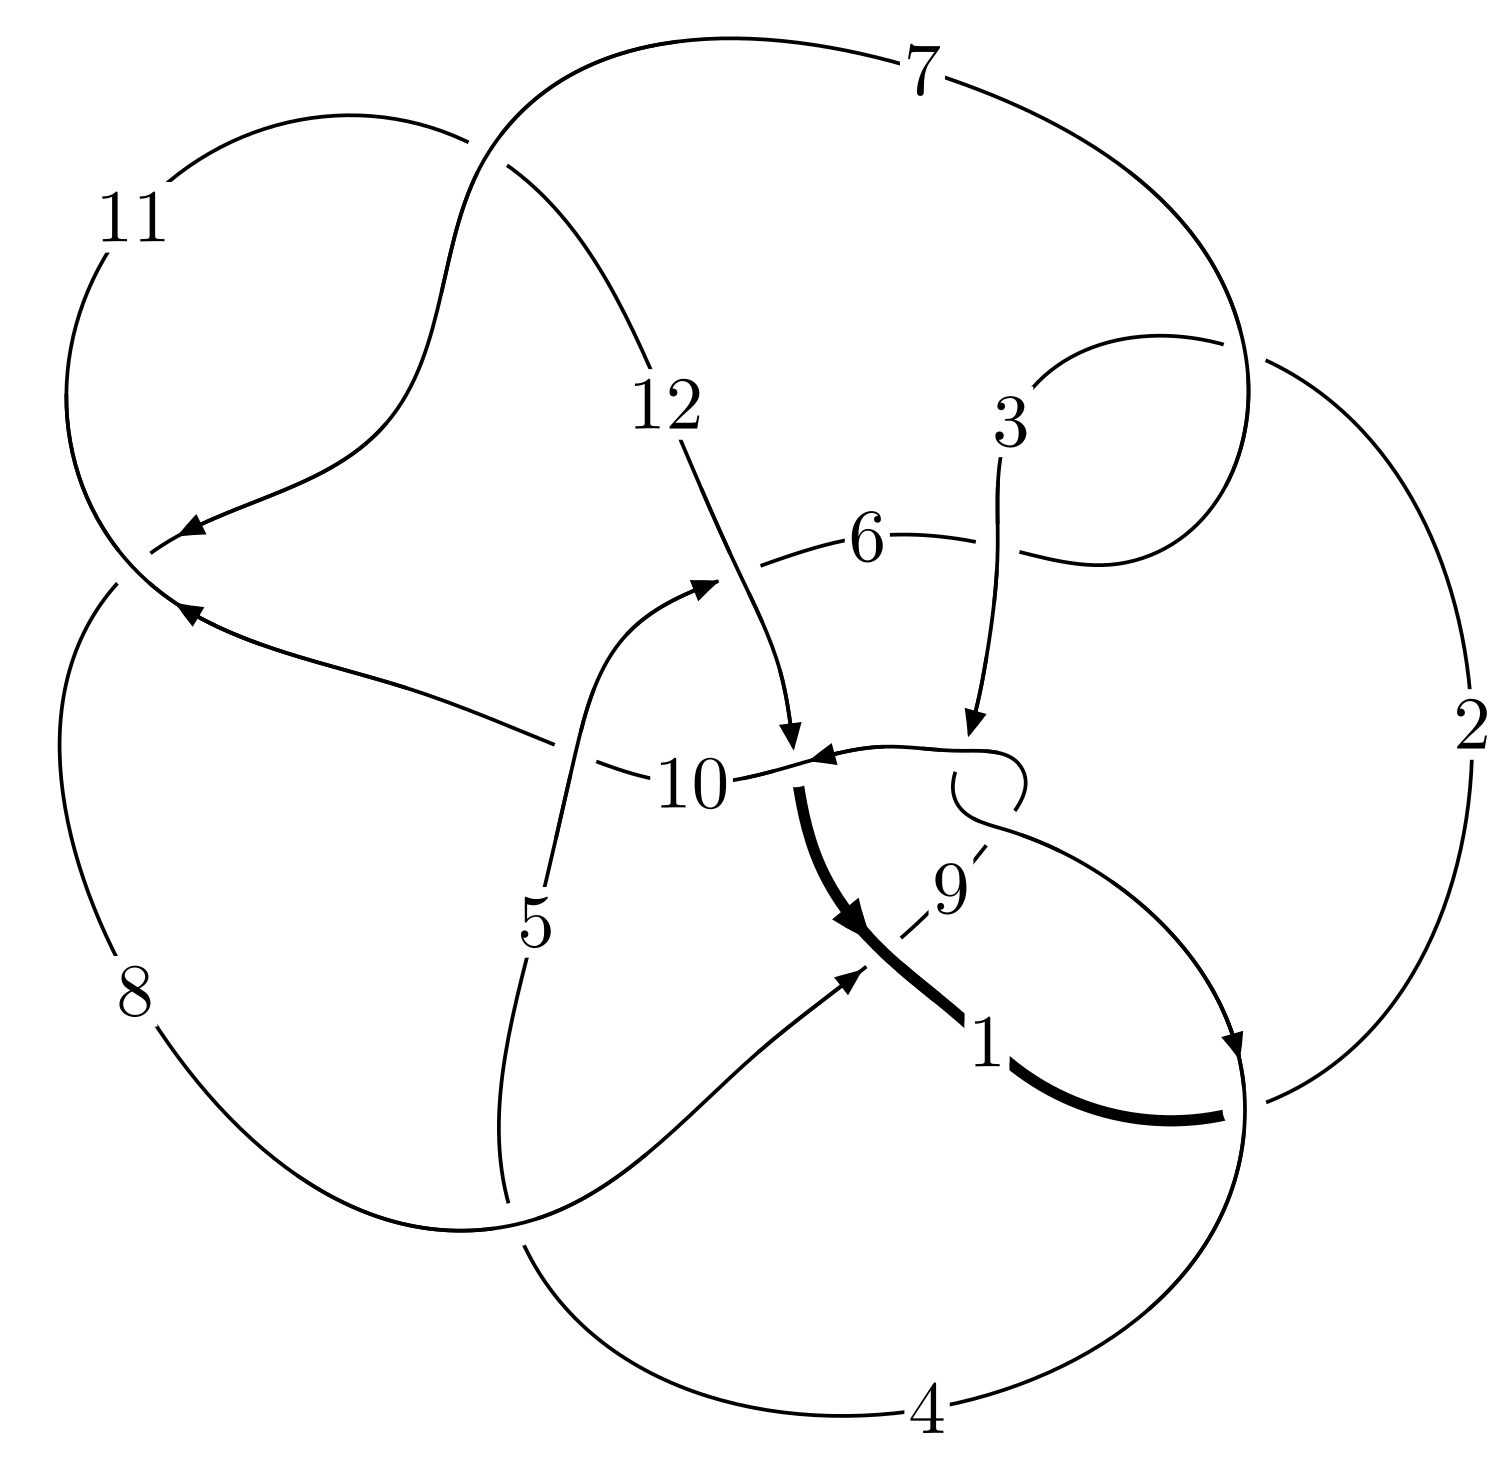
\includegraphics[width=112pt]{../../../GIT/diagram.site/Diagrams/png/2853_12n_0764.png}\\
\ \ \ A knot diagram\footnotemark}&
\allowdisplaybreaks
\textbf{Linearized knot diagam} \\
\cline{2-2}
 &
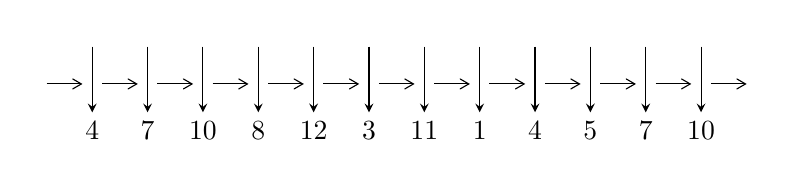
\begin{tikzpicture}[x=20pt, y=17pt]
	% nodes
	\node (C0) at (0, 0) {};
	\node (C1) at (1, 0) {};
	\node (C1U) at (1, +1) {};
	\node (C1D) at (1, -1) {4};

	\node (C2) at (2, 0) {};
	\node (C2U) at (2, +1) {};
	\node (C2D) at (2, -1) {7};

	\node (C3) at (3, 0) {};
	\node (C3U) at (3, +1) {};
	\node (C3D) at (3, -1) {10};

	\node (C4) at (4, 0) {};
	\node (C4U) at (4, +1) {};
	\node (C4D) at (4, -1) {8};

	\node (C5) at (5, 0) {};
	\node (C5U) at (5, +1) {};
	\node (C5D) at (5, -1) {12};

	\node (C6) at (6, 0) {};
	\node (C6U) at (6, +1) {};
	\node (C6D) at (6, -1) {3};

	\node (C7) at (7, 0) {};
	\node (C7U) at (7, +1) {};
	\node (C7D) at (7, -1) {11};

	\node (C8) at (8, 0) {};
	\node (C8U) at (8, +1) {};
	\node (C8D) at (8, -1) {1};

	\node (C9) at (9, 0) {};
	\node (C9U) at (9, +1) {};
	\node (C9D) at (9, -1) {4};

	\node (C10) at (10, 0) {};
	\node (C10U) at (10, +1) {};
	\node (C10D) at (10, -1) {5};

	\node (C11) at (11, 0) {};
	\node (C11U) at (11, +1) {};
	\node (C11D) at (11, -1) {7};

	\node (C12) at (12, 0) {};
	\node (C12U) at (12, +1) {};
	\node (C12D) at (12, -1) {10};
	\node (C13) at (13, 0) {};

	% arrows
	\draw[->,>={angle 60}]
	(C0) edge (C1) (C1) edge (C2) (C2) edge (C3) (C3) edge (C4) (C4) edge (C5) (C5) edge (C6) (C6) edge (C7) (C7) edge (C8) (C8) edge (C9) (C9) edge (C10) (C10) edge (C11) (C11) edge (C12) (C12) edge (C13) ;	\draw[->,>=stealth]
	(C1U) edge (C1D) (C2U) edge (C2D) (C3U) edge (C3D) (C4U) edge (C4D) (C5U) edge (C5D) (C6U) edge (C6D) (C7U) edge (C7D) (C8U) edge (C8D) (C9U) edge (C9D) (C10U) edge (C10D) (C11U) edge (C11D) (C12U) edge (C12D) ;
	\end{tikzpicture} \\
\hhline{~~} \\& 
\textbf{Solving Sequence} \\ \cline{2-2} 
 &
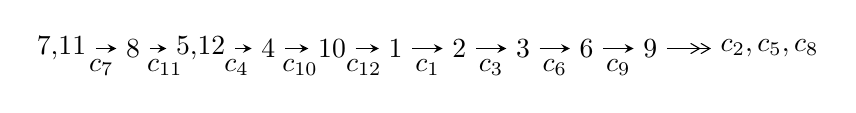
\begin{tikzpicture}[x=23pt, y=7pt]
	% node
	\node (A0) at (-1/8, 0) {7,11};
	\node (A1) at (1, 0) {8};
	\node (A2) at (33/16, 0) {5,12};
	\node (A3) at (25/8, 0) {4};
	\node (A4) at (33/8, 0) {10};
	\node (A5) at (41/8, 0) {1};
	\node (A6) at (49/8, 0) {2};
	\node (A7) at (57/8, 0) {3};
	\node (A8) at (65/8, 0) {6};
	\node (A9) at (73/8, 0) {9};
	\node (C1) at (1/2, -1) {$c_{7}$};
	\node (C2) at (3/2, -1) {$c_{11}$};
	\node (C3) at (21/8, -1) {$c_{4}$};
	\node (C4) at (29/8, -1) {$c_{10}$};
	\node (C5) at (37/8, -1) {$c_{12}$};
	\node (C6) at (45/8, -1) {$c_{1}$};
	\node (C7) at (53/8, -1) {$c_{3}$};
	\node (C8) at (61/8, -1) {$c_{6}$};
	\node (C9) at (69/8, -1) {$c_{9}$};
	\node (A10) at (11, 0) {$c_{2},c_{5},c_{8}$};

	% edge
	\draw[->,>=stealth]	
	(A0) edge (A1) (A1) edge (A2) (A2) edge (A3) (A3) edge (A4) (A4) edge (A5) (A5) edge (A6) (A6) edge (A7) (A7) edge (A8) (A8) edge (A9) ;
	\draw[->>,>={angle 60}]	
	(A9) edge (A10);
\end{tikzpicture} \\ 

\end{tabular} \\

\footnotetext{
The image of knot diagram is generated by the software ``\textbf{Draw programme}" developed by Andrew Bartholomew(\url{http://www.layer8.co.uk/maths/draw/index.htm\#Running-draw}), where we modified some parts for our purpose(\url{https://github.com/CATsTAILs/LinksPainter}).
}\phantom \\ \newline 
\centering \textbf{Ideals for irreducible components\footnotemark of $X_{\text{par}}$} 
 
\begin{align*}
I^u_{1}&=\langle 
-521239 u^{17}-378608 u^{16}+\cdots+1930047 b+369959,\\
\phantom{I^u_{1}}&\phantom{= \langle  }-4207072 u^{17}-369959 u^{16}+\cdots+1930047 a+27427427,\;u^{18}+9 u^{16}+\cdots-7 u+1\rangle \\
I^u_{2}&=\langle 
u^2+b,\;u^6- u^5+2 u^4-4 u^3+u^2+a-2 u+2,\;u^7- u^6+2 u^5-4 u^4+u^3-2 u^2+u+1\rangle \\
I^u_{3}&=\langle 
-47 u^{11}-232 u^{10}+\cdots+125 b-849,\;3669 u^{11}+13414 u^{10}+\cdots+14875 a+13098,\\
\phantom{I^u_{3}}&\phantom{= \langle  }u^{12}+2 u^{11}+8 u^{10}+12 u^9+29 u^8+33 u^7+54 u^6+51 u^5+54 u^4+43 u^3+28 u^2+15 u+7\rangle \\
I^u_{4}&=\langle 
-2931 u^{11}+6882 u^{10}+\cdots+36253 b-67921,\;20673 u^{11}-60690 u^{10}+\cdots+471289 a-219170,\\
\phantom{I^u_{4}}&\phantom{= \langle  }u^{12}-2 u^{11}-2 u^{10}+4 u^9+11 u^8- u^7-6 u^6-7 u^5-14 u^4-19 u^3+10 u^2+25 u+13\rangle \\
\\
\end{align*}
\raggedright * 4 irreducible components of $\dim_{\mathbb{C}}=0$, with total 49 representations.\\
\footnotetext{All coefficients of polynomials are rational numbers. But the coefficients are sometimes approximated in decimal forms when there is not enough margin.}
\newpage
\renewcommand{\arraystretch}{1}
\centering \section*{I. $I^u_{1}= \langle -5.21\times10^{5} u^{17}-3.79\times10^{5} u^{16}+\cdots+1.93\times10^{6} b+3.70\times10^{5},\;-4.21\times10^{6} u^{17}-3.70\times10^{5} u^{16}+\cdots+1.93\times10^{6} a+2.74\times10^{7},\;u^{18}+9 u^{16}+\cdots-7 u+1 \rangle$}
\flushleft \textbf{(i) Arc colorings}\\
\begin{tabular}{m{7pt} m{180pt} m{7pt} m{180pt} }
\flushright $a_{7}=$&$\begin{pmatrix}1\\0\end{pmatrix}$ \\
\flushright $a_{11}=$&$\begin{pmatrix}0\\u\end{pmatrix}$ \\
\flushright $a_{8}=$&$\begin{pmatrix}1\\u^2\end{pmatrix}$ \\
\flushright $a_{5}=$&$\begin{pmatrix}2.17978 u^{17}+0.191684 u^{16}+\cdots+26.2071 u-14.2108\\0.270065 u^{17}+0.196165 u^{16}+\cdots-1.83799 u-0.191684\end{pmatrix}$ \\
\flushright $a_{12}=$&$\begin{pmatrix}- u\\u\end{pmatrix}$ \\
\flushright $a_{4}=$&$\begin{pmatrix}2.17978 u^{17}+0.191684 u^{16}+\cdots+25.2071 u-14.2108\\0.270065 u^{17}+0.196165 u^{16}+\cdots-1.83799 u-0.191684\end{pmatrix}$ \\
\flushright $a_{10}=$&$\begin{pmatrix}-2.64153 u^{17}-0.657915 u^{16}+\cdots-25.4168 u+18.5822\\-0.576170 u^{17}-0.104194 u^{16}+\cdots-0.125886 u+0.849598\end{pmatrix}$ \\
\flushright $a_{1}=$&$\begin{pmatrix}7.90979 u^{17}+1.38868 u^{16}+\cdots+54.3071 u-42.6181\\0.275909 u^{17}+0.141446 u^{16}+\cdots+7.93863 u-3.32710\end{pmatrix}$ \\
\flushright $a_{2}=$&$\begin{pmatrix}2.85131 u^{17}+0.717915 u^{16}+\cdots+18.8121 u-16.5368\\0.0775567 u^{17}-0.0705465 u^{16}+\cdots+6.12764 u-1.93842\end{pmatrix}$ \\
\flushright $a_{3}=$&$\begin{pmatrix}-2.77375 u^{17}-0.788461 u^{16}+\cdots-12.6845 u+14.5983\\-0.0775567 u^{17}+0.0705465 u^{16}+\cdots-6.12764 u+1.93842\end{pmatrix}$ \\
\flushright $a_{6}=$&$\begin{pmatrix}2.06984 u^{17}+0.123529 u^{16}+\cdots+25.9420 u-13.8229\\0.380005 u^{17}+0.264320 u^{16}+\cdots-1.57289 u-0.579533\end{pmatrix}$ \\
\flushright $a_{9}=$&$\begin{pmatrix}-5.96916 u^{17}-1.48818 u^{16}+\cdots-52.2245 u+38.4019\\-0.707998 u^{17}-0.0464724 u^{16}+\cdots-2.87520 u+2.06771\end{pmatrix}$\\&\end{tabular}
\flushleft \textbf{(ii) Obstruction class $= -1$}\\~\\
\flushleft \textbf{(iii) Cusp Shapes $= -\frac{464573}{91907} u^{17}-\frac{454121}{643349} u^{16}+\cdots-\frac{30228500}{643349} u+\frac{10577045}{643349}$}\\~\\
\newpage\renewcommand{\arraystretch}{1}
\flushleft \textbf{(iv) u-Polynomials at the component}\newline \\
\begin{tabular}{m{50pt}|m{274pt}}
Crossings & \hspace{64pt}u-Polynomials at each crossing \\
\hline $$\begin{aligned}c_{1}\end{aligned}$$&$\begin{aligned}
&u^{18}+u^{17}+\cdots+10 u+7
\end{aligned}$\\
\hline $$\begin{aligned}c_{2},c_{6},c_{8}\end{aligned}$$&$\begin{aligned}
&u^{18}+u^{17}+\cdots-3 u-1
\end{aligned}$\\
\hline $$\begin{aligned}c_{3},c_{5},c_{9}\end{aligned}$$&$\begin{aligned}
&u^{18}-16 u^{16}+\cdots-20 u-11
\end{aligned}$\\
\hline $$\begin{aligned}c_{4},c_{7},c_{11}\end{aligned}$$&$\begin{aligned}
&u^{18}+9 u^{16}+\cdots+7 u+1
\end{aligned}$\\
\hline $$\begin{aligned}c_{10}\end{aligned}$$&$\begin{aligned}
&u^{18}+7 u^{17}+\cdots-57 u-7
\end{aligned}$\\
\hline $$\begin{aligned}c_{12}\end{aligned}$$&$\begin{aligned}
&u^{18}-4 u^{17}+\cdots+24 u+117
\end{aligned}$\\
\hline
\end{tabular}\\~\\
\newpage\renewcommand{\arraystretch}{1}
\flushleft \textbf{(v) Riley Polynomials at the component}\newline \\
\begin{tabular}{m{50pt}|m{274pt}}
Crossings & \hspace{64pt}Riley Polynomials at each crossing \\
\hline $$\begin{aligned}c_{1}\end{aligned}$$&$\begin{aligned}
&y^{18}-29 y^{17}+\cdots-1724 y+49
\end{aligned}$\\
\hline $$\begin{aligned}c_{2},c_{6},c_{8}\end{aligned}$$&$\begin{aligned}
&y^{18}-15 y^{17}+\cdots-3 y+1
\end{aligned}$\\
\hline $$\begin{aligned}c_{3},c_{5},c_{9}\end{aligned}$$&$\begin{aligned}
&y^{18}-32 y^{17}+\cdots-1060 y+121
\end{aligned}$\\
\hline $$\begin{aligned}c_{4},c_{7},c_{11}\end{aligned}$$&$\begin{aligned}
&y^{18}+18 y^{17}+\cdots-31 y+1
\end{aligned}$\\
\hline $$\begin{aligned}c_{10}\end{aligned}$$&$\begin{aligned}
&y^{18}+y^{17}+\cdots-337 y+49
\end{aligned}$\\
\hline $$\begin{aligned}c_{12}\end{aligned}$$&$\begin{aligned}
&y^{18}-38 y^{17}+\cdots-200412 y+13689
\end{aligned}$\\
\hline
\end{tabular}\\~\\
\newpage\flushleft \textbf{(vi) Complex Volumes and Cusp Shapes}
$$\begin{array}{c|c|c}  
\text{Solutions to }I^u_{1}& \I (\text{vol} + \sqrt{-1}CS) & \text{Cusp shape}\\
 \hline 
\begin{aligned}
u &= \phantom{-}0.017806 + 1.047910 I \\
a &= \phantom{-}0.678997 - 0.386228 I \\
b &= -0.748794 - 0.598570 I\end{aligned}
 & -0.15119 + 2.09745 I & -12.63201 - 4.12977 I \\ \hline\begin{aligned}
u &= \phantom{-}0.017806 - 1.047910 I \\
a &= \phantom{-}0.678997 + 0.386228 I \\
b &= -0.748794 + 0.598570 I\end{aligned}
 & -0.15119 - 2.09745 I & -12.63201 + 4.12977 I \\ \hline\begin{aligned}
u &= -0.346086 + 0.994636 I \\
a &= -0.819378 + 0.554280 I \\
b &= \phantom{-}1.44016 - 0.91249 I\end{aligned}
 & \phantom{-}5.46595 - 1.70319 I & -1.84461 + 1.40793 I \\ \hline\begin{aligned}
u &= -0.346086 - 0.994636 I \\
a &= -0.819378 - 0.554280 I \\
b &= \phantom{-}1.44016 + 0.91249 I\end{aligned}
 & \phantom{-}5.46595 + 1.70319 I & -1.84461 - 1.40793 I \\ \hline\begin{aligned}
u &= -0.442971 + 1.297020 I \\
a &= -0.306761 - 0.349541 I \\
b &= \phantom{-}0.497178 - 0.425094 I\end{aligned}
 & -0.12898 + 2.98542 I & -11.42448 - 1.55661 I \\ \hline\begin{aligned}
u &= -0.442971 - 1.297020 I \\
a &= -0.306761 + 0.349541 I \\
b &= \phantom{-}0.497178 + 0.425094 I\end{aligned}
 & -0.12898 - 2.98542 I & -11.42448 + 1.55661 I \\ \hline\begin{aligned}
u &= \phantom{-}0.680846 + 1.209390 I \\
a &= \phantom{-}0.815864 - 0.142059 I \\
b &= -1.262000 + 0.276114 I\end{aligned}
 & -0.03662 - 6.82707 I & -12.5292 + 8.6563 I \\ \hline\begin{aligned}
u &= \phantom{-}0.680846 - 1.209390 I \\
a &= \phantom{-}0.815864 + 0.142059 I \\
b &= -1.262000 - 0.276114 I\end{aligned}
 & -0.03662 + 6.82707 I & -12.5292 - 8.6563 I \\ \hline\begin{aligned}
u &= -0.76192 + 1.23703 I \\
a &= \phantom{-}0.045171 - 1.091190 I \\
b &= -1.337910 - 0.285858 I\end{aligned}
 & -13.04820 + 4.46526 I & -11.23742 - 2.32071 I \\ \hline\begin{aligned}
u &= -0.76192 - 1.23703 I \\
a &= \phantom{-}0.045171 + 1.091190 I \\
b &= -1.337910 + 0.285858 I\end{aligned}
 & -13.04820 - 4.46526 I & -11.23742 + 2.32071 I\\
 \hline 
 \end{array}$$\newpage$$\begin{array}{c|c|c}  
\text{Solutions to }I^u_{1}& \I (\text{vol} + \sqrt{-1}CS) & \text{Cusp shape}\\
 \hline 
\begin{aligned}
u &= -0.24569 + 1.44514 I \\
a &= -1.051510 - 0.623676 I \\
b &= \phantom{-}1.93533 + 0.56642 I\end{aligned}
 & \phantom{-}8.63765 + 4.81272 I & -14.8469 + 6.2266 I \\ \hline\begin{aligned}
u &= -0.24569 - 1.44514 I \\
a &= -1.051510 + 0.623676 I \\
b &= \phantom{-}1.93533 - 0.56642 I\end{aligned}
 & \phantom{-}8.63765 - 4.81272 I & -14.8469 - 6.2266 I \\ \hline\begin{aligned}
u &= -0.172111 + 0.488659 I \\
a &= -1.21271 + 2.12963 I \\
b &= \phantom{-}0.783985 - 0.730119 I\end{aligned}
 & \phantom{-}2.63033 - 2.95805 I & -12.64066 + 3.45085 I \\ \hline\begin{aligned}
u &= -0.172111 - 0.488659 I \\
a &= -1.21271 - 2.12963 I \\
b &= \phantom{-}0.783985 + 0.730119 I\end{aligned}
 & \phantom{-}2.63033 + 2.95805 I & -12.64066 - 3.45085 I \\ \hline\begin{aligned}
u &= \phantom{-}0.292901\phantom{ +0.000000I} \\
a &= \phantom{-}1.34245\phantom{ +0.000000I} \\
b &= -0.177730\phantom{ +0.000000I}\end{aligned}
 & -0.535468\phantom{ +0.000000I} & -18.6140\phantom{ +0.000000I} \\ \hline\begin{aligned}
u &= \phantom{-}0.178761\phantom{ +0.000000I} \\
a &= -8.26850\phantom{ +0.000000I} \\
b &= -0.442984\phantom{ +0.000000I}\end{aligned}
 & -7.55325\phantom{ +0.000000I} & \phantom{-}4.27620\phantom{ +0.000000I} \\ \hline\begin{aligned}
u &= \phantom{-}1.03430 + 1.57774 I \\
a &= \phantom{-}0.813344 - 0.058598 I \\
b &= -1.99758 + 1.15997 I\end{aligned}
 & -11.6616 - 12.5169 I & -11.17612 + 5.12731 I \\ \hline\begin{aligned}
u &= \phantom{-}1.03430 - 1.57774 I \\
a &= \phantom{-}0.813344 + 0.058598 I \\
b &= -1.99758 - 1.15997 I\end{aligned}
 & -11.6616 + 12.5169 I & -11.17612 - 5.12731 I\\
 \hline 
 \end{array}$$\newpage\newpage\renewcommand{\arraystretch}{1}
\centering \section*{II. $I^u_{2}= \langle u^2+b,\;u^6- u^5+2 u^4-4 u^3+u^2+a-2 u+2,\;u^7- u^6+2 u^5-4 u^4+u^3-2 u^2+u+1 \rangle$}
\flushleft \textbf{(i) Arc colorings}\\
\begin{tabular}{m{7pt} m{180pt} m{7pt} m{180pt} }
\flushright $a_{7}=$&$\begin{pmatrix}1\\0\end{pmatrix}$ \\
\flushright $a_{11}=$&$\begin{pmatrix}0\\u\end{pmatrix}$ \\
\flushright $a_{8}=$&$\begin{pmatrix}1\\u^2\end{pmatrix}$ \\
\flushright $a_{5}=$&$\begin{pmatrix}- u^6+u^5-2 u^4+4 u^3- u^2+2 u-2\\- u^2\end{pmatrix}$ \\
\flushright $a_{12}=$&$\begin{pmatrix}- u\\u\end{pmatrix}$ \\
\flushright $a_{4}=$&$\begin{pmatrix}- u^6+u^5-2 u^4+4 u^3- u^2+u-2\\- u^3- u^2\end{pmatrix}$ \\
\flushright $a_{10}=$&$\begin{pmatrix}- u^6+u^5-2 u^4+4 u^3- u^2+3 u-3\\u^3- u^2+u\end{pmatrix}$ \\
\flushright $a_{1}=$&$\begin{pmatrix}u^6-2 u^5+5 u^4-9 u^3+8 u^2-10 u+5\\u^6-2 u^5+u^4-4 u^3+u^2+u+1\end{pmatrix}$ \\
\flushright $a_{2}=$&$\begin{pmatrix}u^6- u^5+3 u^4-5 u^3+3 u^2-5 u+2\\u^6- u^5+2 u^4-3 u^3+u^2- u\end{pmatrix}$ \\
\flushright $a_{3}=$&$\begin{pmatrix}u^4-2 u^3+2 u^2-4 u+2\\u^6- u^5+2 u^4-3 u^3+u^2- u\end{pmatrix}$ \\
\flushright $a_{6}=$&$\begin{pmatrix}- u^6+u^5- u^4+4 u^3+u-2\\- u^4-2 u^2+u\end{pmatrix}$ \\
\flushright $a_{9}=$&$\begin{pmatrix}-2 u^6+2 u^5-3 u^4+9 u^3-2 u^2+5 u-6\\u^6+u^5+u^4+u^3-2 u^2+u\end{pmatrix}$\\&\end{tabular}
\flushleft \textbf{(ii) Obstruction class $= 1$}\\~\\
\flushleft \textbf{(iii) Cusp Shapes $= -5 u^6+5 u^5-11 u^4+28 u^3-15 u^2+14 u-24$}\\~\\
\newpage\renewcommand{\arraystretch}{1}
\flushleft \textbf{(iv) u-Polynomials at the component}\newline \\
\begin{tabular}{m{50pt}|m{274pt}}
Crossings & \hspace{64pt}u-Polynomials at each crossing \\
\hline $$\begin{aligned}c_{1}\end{aligned}$$&$\begin{aligned}
&u^7-6 u^5- u^4+9 u^3+u^2-4 u+1
\end{aligned}$\\
\hline $$\begin{aligned}c_{2},c_{8}\end{aligned}$$&$\begin{aligned}
&u^7+2 u^6- u^5+2 u^4+u^3-2 u^2- u-1
\end{aligned}$\\
\hline $$\begin{aligned}c_{3},c_{5}\end{aligned}$$&$\begin{aligned}
&u^7+u^6-5 u^5+5 u^4-9 u^3+7 u^2-1
\end{aligned}$\\
\hline $$\begin{aligned}c_{4},c_{7}\end{aligned}$$&$\begin{aligned}
&u^7- u^6+2 u^5-4 u^4+u^3-2 u^2+u+1
\end{aligned}$\\
\hline $$\begin{aligned}c_{6}\end{aligned}$$&$\begin{aligned}
&u^7-2 u^6- u^5-2 u^4+u^3+2 u^2- u+1
\end{aligned}$\\
\hline $$\begin{aligned}c_{9}\end{aligned}$$&$\begin{aligned}
&u^7- u^6-5 u^5-5 u^4-9 u^3-7 u^2+1
\end{aligned}$\\
\hline $$\begin{aligned}c_{10}\end{aligned}$$&$\begin{aligned}
&u^7+6 u^6+17 u^5+26 u^4+20 u^3+3 u^2-5 u-1
\end{aligned}$\\
\hline $$\begin{aligned}c_{11}\end{aligned}$$&$\begin{aligned}
&u^7+u^6+2 u^5+4 u^4+u^3+2 u^2+u-1
\end{aligned}$\\
\hline $$\begin{aligned}c_{12}\end{aligned}$$&$\begin{aligned}
&u^7+5 u^6+6 u^5+7 u^4+18 u^3+5 u^2+10 u+7
\end{aligned}$\\
\hline
\end{tabular}\\~\\
\newpage\renewcommand{\arraystretch}{1}
\flushleft \textbf{(v) Riley Polynomials at the component}\newline \\
\begin{tabular}{m{50pt}|m{274pt}}
Crossings & \hspace{64pt}Riley Polynomials at each crossing \\
\hline $$\begin{aligned}c_{1}\end{aligned}$$&$\begin{aligned}
&y^7-12 y^6+54 y^5-117 y^4+131 y^3-71 y^2+14 y-1
\end{aligned}$\\
\hline $$\begin{aligned}c_{2},c_{6},c_{8}\end{aligned}$$&$\begin{aligned}
&y^7-6 y^6-5 y^5+15 y^3-2 y^2-3 y-1
\end{aligned}$\\
\hline $$\begin{aligned}c_{3},c_{5},c_{9}\end{aligned}$$&$\begin{aligned}
&y^7-11 y^6-3 y^5+51 y^4+13 y^3-39 y^2+14 y-1
\end{aligned}$\\
\hline $$\begin{aligned}c_{4},c_{7},c_{11}\end{aligned}$$&$\begin{aligned}
&y^7+3 y^6-2 y^5-14 y^4-9 y^3+6 y^2+5 y-1
\end{aligned}$\\
\hline $$\begin{aligned}c_{10}\end{aligned}$$&$\begin{aligned}
&y^7-2 y^6+17 y^5-42 y^4+86 y^3-157 y^2+31 y-1
\end{aligned}$\\
\hline $$\begin{aligned}c_{12}\end{aligned}$$&$\begin{aligned}
&y^7-13 y^6+2 y^5+137 y^4+304 y^3+237 y^2+30 y-49
\end{aligned}$\\
\hline
\end{tabular}\\~\\
\newpage\flushleft \textbf{(vi) Complex Volumes and Cusp Shapes}
$$\begin{array}{c|c|c}  
\text{Solutions to }I^u_{2}& \I (\text{vol} + \sqrt{-1}CS) & \text{Cusp shape}\\
 \hline 
\begin{aligned}
u &= -0.180603 + 0.994309 I \\
a &= -1.17684 - 0.97360 I \\
b &= \phantom{-}0.956033 + 0.359151 I\end{aligned}
 & \phantom{-}3.86399 + 3.81570 I & -7.59315 - 5.07181 I \\ \hline\begin{aligned}
u &= -0.180603 - 0.994309 I \\
a &= -1.17684 + 0.97360 I \\
b &= \phantom{-}0.956033 - 0.359151 I\end{aligned}
 & \phantom{-}3.86399 - 3.81570 I & -7.59315 + 5.07181 I \\ \hline\begin{aligned}
u &= \phantom{-}0.799230\phantom{ +0.000000I} \\
a &= \phantom{-}0.251205\phantom{ +0.000000I} \\
b &= -0.638768\phantom{ +0.000000I}\end{aligned}
 & -3.11260\phantom{ +0.000000I} & -12.2590\phantom{ +0.000000I} \\ \hline\begin{aligned}
u &= \phantom{-}1.42119\phantom{ +0.000000I} \\
a &= -0.296362\phantom{ +0.000000I} \\
b &= -2.01977\phantom{ +0.000000I}\end{aligned}
 & -14.5025\phantom{ +0.000000I} & -11.1100\phantom{ +0.000000I} \\ \hline\begin{aligned}
u &= -0.22015 + 1.41755 I \\
a &= -1.106980 - 0.688829 I \\
b &= \phantom{-}1.96097 + 0.62416 I\end{aligned}
 & \phantom{-}8.82336 + 5.00709 I & \phantom{-}6.2703 - 15.1192 I \\ \hline\begin{aligned}
u &= -0.22015 - 1.41755 I \\
a &= -1.106980 + 0.688829 I \\
b &= \phantom{-}1.96097 - 0.62416 I\end{aligned}
 & \phantom{-}8.82336 - 5.00709 I & \phantom{-}6.2703 + 15.1192 I \\ \hline\begin{aligned}
u &= -0.418901\phantom{ +0.000000I} \\
a &= -3.38720\phantom{ +0.000000I} \\
b &= -0.175478\phantom{ +0.000000I}\end{aligned}
 & -7.75956\phantom{ +0.000000I} & -34.9850\phantom{ +0.000000I}\\
 \hline 
 \end{array}$$\newpage\newpage\renewcommand{\arraystretch}{1}
\centering \section*{III. $I^u_{3}= \langle -47 u^{11}-232 u^{10}+\cdots+125 b-849,\;3669 u^{11}+13414 u^{10}+\cdots+14875 a+13098,\;u^{12}+2 u^{11}+\cdots+15 u+7 \rangle$}
\flushleft \textbf{(i) Arc colorings}\\
\begin{tabular}{m{7pt} m{180pt} m{7pt} m{180pt} }
\flushright $a_{7}=$&$\begin{pmatrix}1\\0\end{pmatrix}$ \\
\flushright $a_{11}=$&$\begin{pmatrix}0\\u\end{pmatrix}$ \\
\flushright $a_{8}=$&$\begin{pmatrix}1\\u^2\end{pmatrix}$ \\
\flushright $a_{5}=$&$\begin{pmatrix}-0.246655 u^{11}-0.901782 u^{10}+\cdots-4.03341 u-0.880538\\0.376000 u^{11}+1.85600 u^{10}+\cdots+17.0880 u+6.79200\end{pmatrix}$ \\
\flushright $a_{12}=$&$\begin{pmatrix}- u\\u\end{pmatrix}$ \\
\flushright $a_{4}=$&$\begin{pmatrix}-0.154420 u^{11}-0.00719328 u^{10}+\cdots+5.20094 u+3.05217\\0.287059 u^{11}+0.957647 u^{10}+\cdots+5.79059 u+1.82118\end{pmatrix}$ \\
\flushright $a_{10}=$&$\begin{pmatrix}0.389513 u^{11}+1.18750 u^{10}+\cdots+8.03341 u+3.02339\\-0.301647 u^{11}-0.798118 u^{10}+\cdots-5.36847 u-3.08094\end{pmatrix}$ \\
\flushright $a_{1}=$&$\begin{pmatrix}0.154420 u^{11}+0.00719328 u^{10}+\cdots-5.20094 u-3.05217\\-0.187294 u^{11}-0.500235 u^{10}+\cdots-2.12894 u+0.310118\end{pmatrix}$ \\
\flushright $a_{2}=$&$\begin{pmatrix}0.0135126 u^{11}+0.331496 u^{10}+\cdots+5.94541 u+2.23139\\0.362824 u^{11}+0.871059 u^{10}+\cdots+4.34024 u+0.944471\end{pmatrix}$ \\
\flushright $a_{3}=$&$\begin{pmatrix}-0.349311 u^{11}-0.539563 u^{10}+\cdots+1.60518 u+1.28692\\0.362824 u^{11}+0.871059 u^{10}+\cdots+4.34024 u+0.944471\end{pmatrix}$ \\
\flushright $a_{6}=$&$\begin{pmatrix}-0.346420 u^{11}-0.359193 u^{10}+\cdots+7.30494 u+3.98817\\0.475765 u^{11}+1.31341 u^{10}+\cdots+5.74965 u+1.92329\end{pmatrix}$ \\
\flushright $a_{9}=$&$\begin{pmatrix}0.778958 u^{11}+1.90568 u^{10}+\cdots+5.02729 u+1.17002\\-0.515765 u^{11}-1.55341 u^{10}+\cdots-5.26965 u-1.60329\end{pmatrix}$\\&\end{tabular}
\flushleft \textbf{(ii) Obstruction class $= 1$}\\~\\
\flushleft \textbf{(iii) Cusp Shapes $= \frac{3466}{2125} u^{11}+\frac{5146}{2125} u^{10}+\frac{20662}{2125} u^9+\frac{4013}{425} u^8+\frac{54149}{2125} u^7+\frac{27374}{2125} u^6+\frac{10937}{425} u^5+\frac{7631}{2125} u^4+\frac{2288}{2125} u^3-\frac{3202}{425} u^2-\frac{16867}{2125} u-\frac{37678}{2125}$}\\~\\
\newpage\renewcommand{\arraystretch}{1}
\flushleft \textbf{(iv) u-Polynomials at the component}\newline \\
\begin{tabular}{m{50pt}|m{274pt}}
Crossings & \hspace{64pt}u-Polynomials at each crossing \\
\hline $$\begin{aligned}c_{1}\end{aligned}$$&$\begin{aligned}
&(u^3-3 u^2+2 u+1)^4
\end{aligned}$\\
\hline $$\begin{aligned}c_{2},c_{8}\end{aligned}$$&$\begin{aligned}
&u^{12}- u^{11}- u^{10}+u^9- u^8+2 u^7+u^6-9 u^5+15 u^4-13 u^3+9 u^2-4 u+1
\end{aligned}$\\
\hline $$\begin{aligned}c_{3},c_{5}\end{aligned}$$&$\begin{aligned}
&u^{12}+4 u^{11}+\cdots+2 u+1
\end{aligned}$\\
\hline $$\begin{aligned}c_{4},c_{7}\end{aligned}$$&$\begin{aligned}
&u^{12}+2 u^{11}+\cdots+15 u+7
\end{aligned}$\\
\hline $$\begin{aligned}c_{6}\end{aligned}$$&$\begin{aligned}
&u^{12}+u^{11}- u^{10}- u^9- u^8-2 u^7+u^6+9 u^5+15 u^4+13 u^3+9 u^2+4 u+1
\end{aligned}$\\
\hline $$\begin{aligned}c_{9}\end{aligned}$$&$\begin{aligned}
&u^{12}-4 u^{11}+\cdots-2 u+1
\end{aligned}$\\
\hline $$\begin{aligned}c_{10}\end{aligned}$$&$\begin{aligned}
&(u^2- u+1)^6
\end{aligned}$\\
\hline $$\begin{aligned}c_{11}\end{aligned}$$&$\begin{aligned}
&u^{12}-2 u^{11}+\cdots-15 u+7
\end{aligned}$\\
\hline $$\begin{aligned}c_{12}\end{aligned}$$&$\begin{aligned}
&u^{12}-4 u^{11}+\cdots+21 u+7
\end{aligned}$\\
\hline
\end{tabular}\\~\\
\newpage\renewcommand{\arraystretch}{1}
\flushleft \textbf{(v) Riley Polynomials at the component}\newline \\
\begin{tabular}{m{50pt}|m{274pt}}
Crossings & \hspace{64pt}Riley Polynomials at each crossing \\
\hline $$\begin{aligned}c_{1}\end{aligned}$$&$\begin{aligned}
&(y^3-5 y^2+10 y-1)^4
\end{aligned}$\\
\hline $$\begin{aligned}c_{2},c_{6},c_{8}\end{aligned}$$&$\begin{aligned}
&y^{12}-3 y^{11}+\cdots+2 y+1
\end{aligned}$\\
\hline $$\begin{aligned}c_{3},c_{5},c_{9}\end{aligned}$$&$\begin{aligned}
&y^{12}-2 y^{11}+\cdots+26 y+1
\end{aligned}$\\
\hline $$\begin{aligned}c_{4},c_{7},c_{11}\end{aligned}$$&$\begin{aligned}
&y^{12}+12 y^{11}+\cdots+167 y+49
\end{aligned}$\\
\hline $$\begin{aligned}c_{10}\end{aligned}$$&$\begin{aligned}
&(y^2+y+1)^6
\end{aligned}$\\
\hline $$\begin{aligned}c_{12}\end{aligned}$$&$\begin{aligned}
&y^{12}+4 y^{11}+\cdots+105 y+49
\end{aligned}$\\
\hline
\end{tabular}\\~\\
\newpage\flushleft \textbf{(vi) Complex Volumes and Cusp Shapes}
$$\begin{array}{c|c|c}  
\text{Solutions to }I^u_{3}& \I (\text{vol} + \sqrt{-1}CS) & \text{Cusp shape}\\
 \hline 
\begin{aligned}
u &= \phantom{-}0.180135 + 0.927755 I \\
a &= \phantom{-}0.798712 + 0.694015 I \\
b &= -1.29718 + 1.09845 I\end{aligned}
 & \phantom{-}0.265740 - 0.798239 I & -10.21508 - 2.15696 I \\ \hline\begin{aligned}
u &= \phantom{-}0.180135 - 0.927755 I \\
a &= \phantom{-}0.798712 - 0.694015 I \\
b &= -1.29718 - 1.09845 I\end{aligned}
 & \phantom{-}0.265740 + 0.798239 I & -10.21508 + 2.15696 I \\ \hline\begin{aligned}
u &= -0.206453 + 1.188860 I \\
a &= -0.636230 + 0.531056 I \\
b &= \phantom{-}1.80380 - 0.74655 I\end{aligned}
 & \phantom{-}4.40332 - 2.02988 I & -10.56984 + 3.46410 I \\ \hline\begin{aligned}
u &= -0.206453 - 1.188860 I \\
a &= -0.636230 - 0.531056 I \\
b &= \phantom{-}1.80380 + 0.74655 I\end{aligned}
 & \phantom{-}4.40332 + 2.02988 I & -10.56984 - 3.46410 I \\ \hline\begin{aligned}
u &= \phantom{-}0.300960 + 1.170050 I \\
a &= -0.797324 + 0.222244 I \\
b &= \phantom{-}1.87013 + 0.59068 I\end{aligned}
 & \phantom{-}0.26574 - 4.85801 I & -10.21508 + 4.77124 I \\ \hline\begin{aligned}
u &= \phantom{-}0.300960 - 1.170050 I \\
a &= -0.797324 - 0.222244 I \\
b &= \phantom{-}1.87013 - 0.59068 I\end{aligned}
 & \phantom{-}0.26574 + 4.85801 I & -10.21508 - 4.77124 I \\ \hline\begin{aligned}
u &= -0.670986 + 0.330909 I \\
a &= \phantom{-}0.087396 + 1.333780 I \\
b &= \phantom{-}0.828521 - 0.773223 I\end{aligned}
 & \phantom{-}4.40332 - 2.02988 I & -10.56984 + 3.46410 I \\ \hline\begin{aligned}
u &= -0.670986 - 0.330909 I \\
a &= \phantom{-}0.087396 - 1.333780 I \\
b &= \phantom{-}0.828521 + 0.773223 I\end{aligned}
 & \phantom{-}4.40332 + 2.02988 I & -10.56984 - 3.46410 I \\ \hline\begin{aligned}
u &= \phantom{-}0.40365 + 1.40633 I \\
a &= -0.663216 + 0.165175 I \\
b &= \phantom{-}0.835953 - 0.124983 I\end{aligned}
 & \phantom{-}0.265740 + 0.798239 I & -10.21508 + 2.15696 I \\ \hline\begin{aligned}
u &= \phantom{-}0.40365 - 1.40633 I \\
a &= -0.663216 - 0.165175 I \\
b &= \phantom{-}0.835953 + 0.124983 I\end{aligned}
 & \phantom{-}0.265740 - 0.798239 I & -10.21508 - 2.15696 I\\
 \hline 
 \end{array}$$\newpage$$\begin{array}{c|c|c}  
\text{Solutions to }I^u_{3}& \I (\text{vol} + \sqrt{-1}CS) & \text{Cusp shape}\\
 \hline 
\begin{aligned}
u &= -1.00731 + 1.43634 I \\
a &= \phantom{-}0.567805 - 0.050096 I \\
b &= -1.041220 - 0.420474 I\end{aligned}
 & \phantom{-}0.26574 + 4.85801 I & -10.21508 - 4.77124 I \\ \hline\begin{aligned}
u &= -1.00731 - 1.43634 I \\
a &= \phantom{-}0.567805 + 0.050096 I \\
b &= -1.041220 + 0.420474 I\end{aligned}
 & \phantom{-}0.26574 - 4.85801 I & -10.21508 + 4.77124 I\\
 \hline 
 \end{array}$$\newpage\newpage\renewcommand{\arraystretch}{1}
\centering \section*{IV. $I^u_{4}= \langle -2931 u^{11}+6882 u^{10}+\cdots+36253 b-67921,\;20673 u^{11}-60690 u^{10}+\cdots+471289 a-219170,\;u^{12}-2 u^{11}+\cdots+25 u+13 \rangle$}
\flushleft \textbf{(i) Arc colorings}\\
\begin{tabular}{m{7pt} m{180pt} m{7pt} m{180pt} }
\flushright $a_{7}=$&$\begin{pmatrix}1\\0\end{pmatrix}$ \\
\flushright $a_{11}=$&$\begin{pmatrix}0\\u\end{pmatrix}$ \\
\flushright $a_{8}=$&$\begin{pmatrix}1\\u^2\end{pmatrix}$ \\
\flushright $a_{5}=$&$\begin{pmatrix}-0.0438648 u^{11}+0.128774 u^{10}+\cdots-0.996698 u+0.465044\\0.0808485 u^{11}-0.189833 u^{10}+\cdots+2.60001 u+1.87353\end{pmatrix}$ \\
\flushright $a_{12}=$&$\begin{pmatrix}- u\\u\end{pmatrix}$ \\
\flushright $a_{4}=$&$\begin{pmatrix}0.0941100 u^{11}-0.160829 u^{10}+\cdots+2.05919 u+2.87215\\0.0281356 u^{11}+0.0393623 u^{10}+\cdots+1.14768 u+2.05103\end{pmatrix}$ \\
\flushright $a_{10}=$&$\begin{pmatrix}0.120788 u^{11}-0.282621 u^{10}+\cdots+1.76593 u+1.45803\\0.0273908 u^{11}-0.164621 u^{10}+\cdots+0.519405 u-1.22343\end{pmatrix}$ \\
\flushright $a_{1}=$&$\begin{pmatrix}-0.0941100 u^{11}+0.160829 u^{10}+\cdots-2.05919 u-2.87215\\-0.0324939 u^{11}+0.0685461 u^{10}+\cdots+0.472016 u-0.826442\end{pmatrix}$ \\
\flushright $a_{2}=$&$\begin{pmatrix}-0.133483 u^{11}+0.361165 u^{10}+\cdots-2.47857 u-2.33702\\-0.190081 u^{11}+0.415166 u^{10}+\cdots-2.22379 u-2.79433\end{pmatrix}$ \\
\flushright $a_{3}=$&$\begin{pmatrix}-0.0565980 u^{11}+0.0540008 u^{10}+\cdots+0.254780 u-0.457318\\0.190081 u^{11}-0.415166 u^{10}+\cdots+2.22379 u+2.79433\end{pmatrix}$ \\
\flushright $a_{6}=$&$\begin{pmatrix}0.108895 u^{11}-0.270117 u^{10}+\cdots-0.193179 u+0.632864\\-0.0719113 u^{11}+0.209059 u^{10}+\cdots+1.79649 u+1.70571\end{pmatrix}$ \\
\flushright $a_{9}=$&$\begin{pmatrix}0.177965 u^{11}-0.558920 u^{10}+\cdots+2.12679 u+1.81136\\0.514054 u^{11}-1.53965 u^{10}+\cdots+9.23946 u+4.75588\end{pmatrix}$\\&\end{tabular}
\flushleft \textbf{(ii) Obstruction class $= -1$}\\~\\
\flushleft \textbf{(iii) Cusp Shapes $= -\frac{3530}{36253} u^{11}+\frac{19484}{36253} u^{10}-\frac{23246}{36253} u^9-\frac{11803}{36253} u^8-\frac{17415}{36253} u^7+\frac{113796}{36253} u^6+\frac{5597}{36253} u^5+\frac{68101}{36253} u^4-\frac{58140}{36253} u^3-\frac{1074}{36253} u^2-\frac{209035}{36253} u-\frac{58638}{5179}$}\\~\\
\newpage\renewcommand{\arraystretch}{1}
\flushleft \textbf{(iv) u-Polynomials at the component}\newline \\
\begin{tabular}{m{50pt}|m{274pt}}
Crossings & \hspace{64pt}u-Polynomials at each crossing \\
\hline $$\begin{aligned}c_{1}\end{aligned}$$&$\begin{aligned}
&(u^3- u^2-2 u+1)^4
\end{aligned}$\\
\hline $$\begin{aligned}c_{2},c_{6},c_{8}\end{aligned}$$&$\begin{aligned}
&u^{12}+u^{11}+\cdots-308 u+91
\end{aligned}$\\
\hline $$\begin{aligned}c_{3},c_{5},c_{9}\end{aligned}$$&$\begin{aligned}
&u^{12}+4 u^{11}+\cdots+315 u^2+189
\end{aligned}$\\
\hline $$\begin{aligned}c_{4},c_{7},c_{11}\end{aligned}$$&$\begin{aligned}
&u^{12}+2 u^{11}+\cdots-25 u+13
\end{aligned}$\\
\hline $$\begin{aligned}c_{10}\end{aligned}$$&$\begin{aligned}
&(u^2- u+1)^6
\end{aligned}$\\
\hline $$\begin{aligned}c_{12}\end{aligned}$$&$\begin{aligned}
&u^{12}-18 u^{10}+\cdots-525 u+127
\end{aligned}$\\
\hline
\end{tabular}\\~\\
\newpage\renewcommand{\arraystretch}{1}
\flushleft \textbf{(v) Riley Polynomials at the component}\newline \\
\begin{tabular}{m{50pt}|m{274pt}}
Crossings & \hspace{64pt}Riley Polynomials at each crossing \\
\hline $$\begin{aligned}c_{1}\end{aligned}$$&$\begin{aligned}
&(y^3-5 y^2+6 y-1)^4
\end{aligned}$\\
\hline $$\begin{aligned}c_{2},c_{6},c_{8}\end{aligned}$$&$\begin{aligned}
&y^{12}-31 y^{11}+\cdots-27342 y+8281
\end{aligned}$\\
\hline $$\begin{aligned}c_{3},c_{5},c_{9}\end{aligned}$$&$\begin{aligned}
&y^{12}-38 y^{11}+\cdots+119070 y+35721
\end{aligned}$\\
\hline $$\begin{aligned}c_{4},c_{7},c_{11}\end{aligned}$$&$\begin{aligned}
&y^{12}-8 y^{11}+\cdots-365 y+169
\end{aligned}$\\
\hline $$\begin{aligned}c_{10}\end{aligned}$$&$\begin{aligned}
&(y^2+y+1)^6
\end{aligned}$\\
\hline $$\begin{aligned}c_{12}\end{aligned}$$&$\begin{aligned}
&y^{12}-36 y^{11}+\cdots-25943 y+16129
\end{aligned}$\\
\hline
\end{tabular}\\~\\
\newpage\flushleft \textbf{(vi) Complex Volumes and Cusp Shapes}
$$\begin{array}{c|c|c}  
\text{Solutions to }I^u_{4}& \I (\text{vol} + \sqrt{-1}CS) & \text{Cusp shape}\\
 \hline 
\begin{aligned}
u &= -0.935871 + 0.612228 I \\
a &= \phantom{-}0.798080 - 0.403281 I \\
b &= -1.27562 - 0.98498 I\end{aligned}
 & -3.05488 + 2.02988 I & -11.80194 - 3.46410 I \\ \hline\begin{aligned}
u &= -0.935871 - 0.612228 I \\
a &= \phantom{-}0.798080 + 0.403281 I \\
b &= -1.27562 + 0.98498 I\end{aligned}
 & -3.05488 - 2.02988 I & -11.80194 + 3.46410 I \\ \hline\begin{aligned}
u &= \phantom{-}0.267965 + 1.122990 I \\
a &= -0.830154 + 0.247151 I \\
b &= \phantom{-}1.50749 - 0.36507 I\end{aligned}
 & \phantom{-}2.58490 - 2.02988 I & -8.75302 + 3.46410 I \\ \hline\begin{aligned}
u &= \phantom{-}0.267965 - 1.122990 I \\
a &= -0.830154 - 0.247151 I \\
b &= \phantom{-}1.50749 + 0.36507 I\end{aligned}
 & \phantom{-}2.58490 + 2.02988 I & -8.75302 - 3.46410 I \\ \hline\begin{aligned}
u &= -0.668934 + 0.428490 I \\
a &= \phantom{-}1.118010 - 0.578487 I \\
b &= -0.304581 + 0.329429 I\end{aligned}
 & \phantom{-}2.58490 + 2.02988 I & -8.75302 - 3.46410 I \\ \hline\begin{aligned}
u &= -0.668934 - 0.428490 I \\
a &= \phantom{-}1.118010 + 0.578487 I \\
b &= -0.304581 - 0.329429 I\end{aligned}
 & \phantom{-}2.58490 - 2.02988 I & -8.75302 + 3.46410 I \\ \hline\begin{aligned}
u &= \phantom{-}1.213350 + 0.131620 I \\
a &= -0.483814 - 0.661265 I \\
b &= \phantom{-}0.443182 - 0.504374 I\end{aligned}
 & -3.05488 - 2.02988 I & -11.80194 + 3.46410 I \\ \hline\begin{aligned}
u &= \phantom{-}1.213350 - 0.131620 I \\
a &= -0.483814 + 0.661265 I \\
b &= \phantom{-}0.443182 + 0.504374 I\end{aligned}
 & -3.05488 + 2.02988 I & -11.80194 - 3.46410 I \\ \hline\begin{aligned}
u &= -0.894944 + 0.895021 I \\
a &= \phantom{-}0.763167 - 0.204455 I \\
b &= -2.34607 - 2.27347 I\end{aligned}
 & -14.3344 + 2.0299 I & -10.44504 - 3.46410 I \\ \hline\begin{aligned}
u &= -0.894944 - 0.895021 I \\
a &= \phantom{-}0.763167 + 0.204455 I \\
b &= -2.34607 + 2.27347 I\end{aligned}
 & -14.3344 - 2.0299 I & -10.44504 + 3.46410 I\\
 \hline 
 \end{array}$$\newpage$$\begin{array}{c|c|c}  
\text{Solutions to }I^u_{4}& \I (\text{vol} + \sqrt{-1}CS) & \text{Cusp shape}\\
 \hline 
\begin{aligned}
u &= \phantom{-}2.01843 + 1.05092 I \\
a &= -0.019135 + 0.439021 I \\
b &= -1.024400 + 0.327533 I\end{aligned}
 & -14.3344 + 2.0299 I & -10.44504 - 3.46410 I \\ \hline\begin{aligned}
u &= \phantom{-}2.01843 - 1.05092 I \\
a &= -0.019135 - 0.439021 I \\
b &= -1.024400 - 0.327533 I\end{aligned}
 & -14.3344 - 2.0299 I & -10.44504 + 3.46410 I\\
 \hline 
 \end{array}$$\newpage
\newpage\renewcommand{\arraystretch}{1}
\centering \section*{ V. u-Polynomials}
\begin{tabular}{m{50pt}|m{274pt}}
Crossings & \hspace{64pt}u-Polynomials at each crossing \\
\hline $$\begin{aligned}c_{1}\end{aligned}$$&$\begin{aligned}
&(u^3-3 u^2+2 u+1)^4(u^3- u^2-2 u+1)^4\\
&\cdot(u^7-6 u^5- u^4+9 u^3+u^2-4 u+1)(u^{18}+u^{17}+\cdots+10 u+7)
\end{aligned}$\\
\hline $$\begin{aligned}c_{2},c_{8}\end{aligned}$$&$\begin{aligned}
&(u^7+2 u^6- u^5+2 u^4+u^3-2 u^2- u-1)\\
&\cdot(u^{12}- u^{11}- u^{10}+u^9- u^8+2 u^7+u^6-9 u^5+15 u^4-13 u^3+9 u^2-4 u+1)\\
&\cdot(u^{12}+u^{11}+\cdots-308 u+91)(u^{18}+u^{17}+\cdots-3 u-1)
\end{aligned}$\\
\hline $$\begin{aligned}c_{3},c_{5}\end{aligned}$$&$\begin{aligned}
&(u^7+u^6+\cdots+7 u^2-1)(u^{12}+4 u^{11}+\cdots+315 u^2+189)\\
&\cdot(u^{12}+4 u^{11}+\cdots+2 u+1)(u^{18}-16 u^{16}+\cdots-20 u-11)
\end{aligned}$\\
\hline $$\begin{aligned}c_{4},c_{7}\end{aligned}$$&$\begin{aligned}
&(u^7- u^6+\cdots+u+1)(u^{12}+2 u^{11}+\cdots-25 u+13)\\
&\cdot(u^{12}+2 u^{11}+\cdots+15 u+7)(u^{18}+9 u^{16}+\cdots+7 u+1)
\end{aligned}$\\
\hline $$\begin{aligned}c_{6}\end{aligned}$$&$\begin{aligned}
&(u^7-2 u^6+\cdots- u+1)(u^{12}+u^{11}+\cdots-308 u+91)\\
&\cdot(u^{12}+u^{11}- u^{10}- u^9- u^8-2 u^7+u^6+9 u^5+15 u^4+13 u^3+9 u^2+4 u+1)\\
&\cdot(u^{18}+u^{17}+\cdots-3 u-1)
\end{aligned}$\\
\hline $$\begin{aligned}c_{9}\end{aligned}$$&$\begin{aligned}
&(u^7- u^6+\cdots-7 u^2+1)(u^{12}-4 u^{11}+\cdots-2 u+1)\\
&\cdot(u^{12}+4 u^{11}+\cdots+315 u^2+189)(u^{18}-16 u^{16}+\cdots-20 u-11)
\end{aligned}$\\
\hline $$\begin{aligned}c_{10}\end{aligned}$$&$\begin{aligned}
&(u^2- u+1)^{12}(u^7+6 u^6+17 u^5+26 u^4+20 u^3+3 u^2-5 u-1)\\
&\cdot(u^{18}+7 u^{17}+\cdots-57 u-7)
\end{aligned}$\\
\hline $$\begin{aligned}c_{11}\end{aligned}$$&$\begin{aligned}
&(u^7+u^6+\cdots+u-1)(u^{12}-2 u^{11}+\cdots-15 u+7)\\
&\cdot(u^{12}+2 u^{11}+\cdots-25 u+13)(u^{18}+9 u^{16}+\cdots+7 u+1)
\end{aligned}$\\
\hline $$\begin{aligned}c_{12}\end{aligned}$$&$\begin{aligned}
&(u^7+5 u^6+6 u^5+7 u^4+18 u^3+5 u^2+10 u+7)\\
&\cdot(u^{12}-18 u^{10}+\cdots-525 u+127)(u^{12}-4 u^{11}+\cdots+21 u+7)\\
&\cdot(u^{18}-4 u^{17}+\cdots+24 u+117)
\end{aligned}$\\
\hline
\end{tabular}\newpage\renewcommand{\arraystretch}{1}
\centering \section*{ VI. Riley Polynomials}
\begin{tabular}{m{50pt}|m{274pt}}
Crossings & \hspace{64pt}Riley Polynomials at each crossing \\
\hline $$\begin{aligned}c_{1}\end{aligned}$$&$\begin{aligned}
&(y^3-5 y^2+6 y-1)^4(y^3-5 y^2+10 y-1)^4\\
&\cdot(y^7-12 y^6+54 y^5-117 y^4+131 y^3-71 y^2+14 y-1)\\
&\cdot(y^{18}-29 y^{17}+\cdots-1724 y+49)
\end{aligned}$\\
\hline $$\begin{aligned}c_{2},c_{6},c_{8}\end{aligned}$$&$\begin{aligned}
&(y^7-6 y^6-5 y^5+15 y^3-2 y^2-3 y-1)\\
&\cdot(y^{12}-31 y^{11}+\cdots-27342 y+8281)(y^{12}-3 y^{11}+\cdots+2 y+1)\\
&\cdot(y^{18}-15 y^{17}+\cdots-3 y+1)
\end{aligned}$\\
\hline $$\begin{aligned}c_{3},c_{5},c_{9}\end{aligned}$$&$\begin{aligned}
&(y^7-11 y^6-3 y^5+51 y^4+13 y^3-39 y^2+14 y-1)\\
&\cdot(y^{12}-38 y^{11}+\cdots+119070 y+35721)(y^{12}-2 y^{11}+\cdots+26 y+1)\\
&\cdot(y^{18}-32 y^{17}+\cdots-1060 y+121)
\end{aligned}$\\
\hline $$\begin{aligned}c_{4},c_{7},c_{11}\end{aligned}$$&$\begin{aligned}
&(y^7+3 y^6-2 y^5-14 y^4-9 y^3+6 y^2+5 y-1)\\
&\cdot(y^{12}-8 y^{11}+\cdots-365 y+169)(y^{12}+12 y^{11}+\cdots+167 y+49)\\
&\cdot(y^{18}+18 y^{17}+\cdots-31 y+1)
\end{aligned}$\\
\hline $$\begin{aligned}c_{10}\end{aligned}$$&$\begin{aligned}
&(y^2+y+1)^{12}(y^7-2 y^6+17 y^5-42 y^4+86 y^3-157 y^2+31 y-1)\\
&\cdot(y^{18}+y^{17}+\cdots-337 y+49)
\end{aligned}$\\
\hline $$\begin{aligned}c_{12}\end{aligned}$$&$\begin{aligned}
&(y^7-13 y^6+2 y^5+137 y^4+304 y^3+237 y^2+30 y-49)\\
&\cdot(y^{12}-36 y^{11}+\cdots-25943 y+16129)(y^{12}+4 y^{11}+\cdots+105 y+49)\\
&\cdot(y^{18}-38 y^{17}+\cdots-200412 y+13689)
\end{aligned}$\\
\hline
\end{tabular}
\vskip 2pc
\end{document}